% Compact PGFPlots panel for sampled surface7 BSC bit-scale decomposition.
% Requires \usepackage{pgfplots} and \pgfplotsset{compat=1.18}.
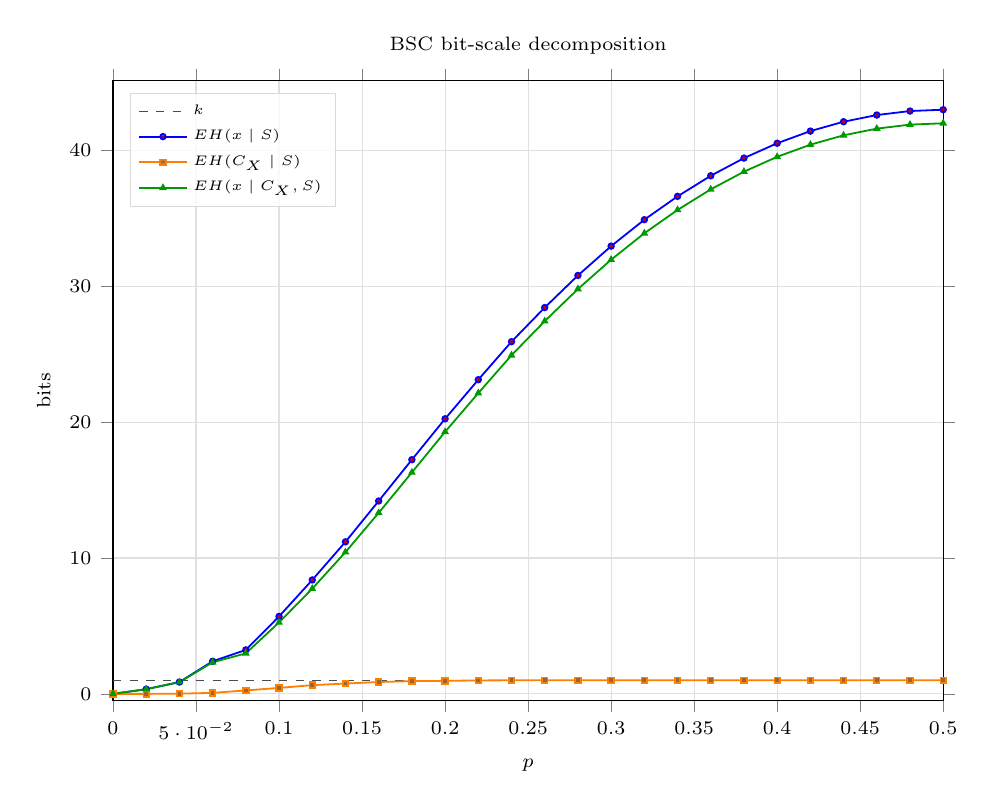
\begin{tikzpicture}
\begin{axis}[
  name=surface7BSCBitScaleAxis,
  width=\linewidth,
  height=0.78\linewidth,
  title={BSC bit-scale decomposition},
  title style={font=\scriptsize},
  xlabel={$p$},
  ylabel={bits},
  xmin=0, xmax=0.5,
  ymin=-0.5, ymax=45.15,
  grid=both,
  major grid style={black!12},
  minor grid style={black!6},
  tick align=outside,
  tick label style={font=\scriptsize},
  label style={font=\scriptsize},
  legend cell align={left},
  legend style={draw=black!15, fill=white, fill opacity=0.82, text opacity=1, at={(0.02,0.98)}, anchor=north west, font=\tiny},
]
\addplot[black!70, dashed, line width=0.55pt] coordinates {(0,1) (0.5,1)};
\addlegendentry{$k$}
\addplot+[color=blue, mark=*, mark size=1.0pt, line width=0.65pt]
coordinates {(0,0) (0.02,0.3447394948) (0.04,0.87228167945) (0.06,2.39882765367) (0.08,3.23572238593) (0.1,5.69954510593) (0.12,8.38569445914) (0.14,11.1910325725) (0.16,14.1969508645) (0.18,17.2376245841) (0.2,20.2472472882) (0.22,23.1266415379) (0.24,25.9241854413) (0.26,28.4343258546) (0.28,30.799801917) (0.3,32.95741289) (0.32,34.9028724659) (0.34,36.6212256022) (0.36,38.1366701514) (0.38,39.4375065958) (0.4,40.5310534686) (0.42,41.4251704131) (0.44,42.11480402) (0.46,42.6072091985) (0.48,42.9018851916) (0.5,43)};
\addlegendentry{$\mathbb{E}H(x\mid S)$}
\addplot+[color=orange, mark=square*, mark size=1.0pt, line width=0.65pt]
coordinates {(0,0) (0.02,4.88963922152e-05) (0.04,0.0131385627784) (0.06,0.0748830555707) (0.08,0.253053194042) (0.1,0.439204807181) (0.12,0.642443213798) (0.14,0.7581302242) (0.16,0.873402626786) (0.18,0.9383546273) (0.2,0.958617090838) (0.22,0.989115981864) (0.24,0.998717069098) (0.26,1.00062140282) (0.28,0.999748563053) (0.3,0.999808539933) (0.32,0.999816448002) (0.34,1.00004349769) (0.36,1.00003080851) (0.38,1.00000510911) (0.4,0.999999852055) (0.42,1.00000076962) (0.44,0.999999993558) (0.46,1.00000000365) (0.48,0.999999999975) (0.5,1)};
\addlegendentry{$\mathbb{E}H(C_X\mid S)$}
\addplot+[color=green!60!black, mark=triangle*, mark size=1.0pt, line width=0.65pt]
coordinates {(0,0) (0.02,0.344690598408) (0.04,0.859143116671) (0.06,2.3239445981) (0.08,2.98266919188) (0.1,5.26034029874) (0.12,7.74325124534) (0.14,10.4329023483) (0.16,13.3235482377) (0.18,16.2992699568) (0.2,19.2886301973) (0.22,22.137525556) (0.24,24.9254683722) (0.26,27.4337044518) (0.28,29.8000533539) (0.3,31.9576043501) (0.32,33.9030560179) (0.34,35.6211821045) (0.36,37.1366393428) (0.38,38.4375014867) (0.4,39.5310536165) (0.42,40.4251696434) (0.44,41.1148040264) (0.46,41.6072091948) (0.48,41.9018851916) (0.5,42)};
\addlegendentry{$\mathbb{E}H(x\mid C_X,S)$}
\end{axis}
\end{tikzpicture}
